\documentclass[10pt,conference,compsocconf]{IEEEtran}

\usepackage{url}
\usepackage{graphicx}	% For figure environment
\usepackage{booktabs}   % For formal tables

\usepackage[utf8]{inputenc}
\usepackage{textcomp}
\usepackage{subcaption}
\captionsetup[subfigure]{skip=0pt}

\usepackage{amsmath}
\usepackage{amssymb}
\usepackage{hyperref}
\usepackage{cleveref}
\usepackage[x11names,svgnames,hyperref,showerrors]{xcolor}

\newcommand{\ra}[1]{\renewcommand{\arraystretch}{#1}}

% \makeatletter
%   \AtBeginDocument{%
%     \def\Ginclude@graphics#1{%
%       \begingroup\fboxsep=-\fboxrule
%       \fbox{\rule{\@ifundefined{Gin@@ewidth}{150pt}{\Gin@@ewidth}}{0pt}%
%         \rule{0pt}{\@ifundefined{Gin@@eheight}{100pt}{\Gin@@eheight}}}\endgroup}}
% \makeatother

\begin{document}
\title{Computational Intelligence Laboratory 2018 \textendash{} Project Report\\{\large Road Segmentation on RGB Satellite Images}}

%SORT ABC
\author{
	\IEEEauthorblockN{
    	Mickey Vänskä\IEEEauthorrefmark{1},
        Jimmy Envall\IEEEauthorrefmark{2},
        Ivan Tishchenko\IEEEauthorrefmark{3},
        Jonathan Granskog\IEEEauthorrefmark{4},
    }
    \IEEEauthorblockA{
  		ETH Zürich\\
  		Zürich, Switzerland\\
        {\IEEEauthorrefmark{1}\href{mailto:mickeyv@student.ethz.ch}{mickeyv@student.ethz.ch}},
        {\IEEEauthorrefmark{2}\href{mailto:jenvall@student.ethz.ch}{jenvall@student.ethz.ch}},
        {\IEEEauthorrefmark{3}\href{mailto:tivan@student.ethz.ch}{tivan@student.ethz.ch}},
        {\IEEEauthorrefmark{3}\href{mailto:granskoj@student.ethz.ch}{granskoj@student.ethz.ch}},
	}
}

\maketitle

\begin{abstract}
    The extraction of information from image and video is one prevalent challenge in computer vision and machine learning.
    A concrete problem is locating and labelling objects in an image, for example during the conversion of satellite images to road maps. In theory this allows map-services to enhance and update their images automatically by detecting new roads from updated satellite images as well as to notify of discrepancies between machine-generated and human-generated predictions.
    Factors such as large variances in road designs, lighting conditions and occlusions make roads surprisingly challenging to categorize correctly.
    This project explores the use of various CNNs for labelling roads in RGB satellite images and concludes the use of a modified ResNet18 to give similar mean F-scores as fully convolutional models.
    A classification network used as a modified segmentation network highlights the adaptability to many tasks having performed equally well to state-of-the-art segmentation networks, such as SegNet and RedNet.
    Although Residual Networks were not designed for the task of image segmentation, they proved to return adequate results when using non-fully-convolutional designs. The results initiate an interesting question on the design of future segmentation networks.
\end{abstract}

\section{Introduction}
\label{sec:introduction}
Smartphone and computer owners can benefit today from a variety of localization services with up-to-date information of their environment. The information that these services rely on is commonly based on current aerial and satellite images. For a single city, this data could possibly be segmented by a single person but this becomes infeasible on a large scale because the segmentation has to be accurate and performed quickly to offer up-to-date information.

In this paper, we survey a variety of neural networks for binary classification of roads in RGB satellite images. All of the methods are based on convolutional neural networks (CNNs) and their performance is compared using a road segmentation competition test set on Kaggle\cite{url:kaggle}.

\section{Related Work}
\label{sec:related-work}
State-of-the-art CNNs for image classification problems are ResNet\cite{he2016deep} and Inception-v4 with Inception-ResNet-v2\cite{szegedy2017inception}. The latter design is an amalgam of the core principles of Inception-v1 and ResNet. Residual Networks are the first successful design of very deep CNNs for image classification that can easily scale to hundreds of layers and adapt to various classification tasks while being robust to vanishing gradients by heavy use of identity connections.

Fundamental work in semantic segmentation by Long et al.\cite{long2015fully} shows that fully convolutional networks can serve as a powerful basis for pixel-wise segmentation. SegNet\cite{badrinarayanan2015segnet} develops the idea further and provides a great framework for pixel-wise multi-class semantic segmentation based on an encoder-decoder architecture inspired by VGG-16\cite{simonyan2014very}. The work on RedNet\cite{jiang2018rednet} demonstrates the use of a residual encoder-decoder architecture using RGB images with depth information for segmentation tasks.

Bittel et al.\cite{bittel2015pixel} applied a fully convolutional architecture for street segmentation. Corentin et al.\cite{henry2018road} proposed a solution to the specific problem of road segmentation from satellite images. Their approach involves a fully convolutional network for pixel-wise segmentation combined with VGG-19\cite{simonyan2014very}.

\section{Models and Methods}
\label{sec:models-and-methods}

Our models are built using Keras-2.2.0\footnote{A problem affecting NCHW batch normalization was discovered in the official release and fixed by us. Our models require this fix.}\cite{url:keras} with Tensorflow-1.7\cite{url:tensorflow} as the backend. Additionally, we use the Python-library imgaug-0.2.5\cite{url:imgaug} for image augmentation.

\subsection{Problem Statement}
\label{subsec:problem-statement}
The data is initially split into two sets, a training and a test set. The training set consists of 100 RGB satellite images of size $400 \times 400$ pixels with grayscale ground-truth maps of the same size. The latter have gradual borders between road and non-road. The test set consists of 94 RGB images of size $608\times 608$.

The set is unbalanced as there is more background than roads in the dataset and therefore a combined F\textsubscript{1}-score
is used as a performance measure. The weights of the two classes are unknown outside of the evaluation system. The goal is thus to construct a classifier that assigns $y \in \{0, 1\}^n$ to a subdivided image $X \in \mathbb{R}^{n\times 3\times 16\times 16}$ such that the combined F\textsubscript{1} is maximized.

The accuracy of the classifier is measured at a granularity of $16\times 16$ pixels. Due to this limit, pixel-wise predictions eventually have to be downsampled. Each patch having marked 25\% or more of its pixels with road is labelled as road, else the patch is marked as background.

\subsection{Model Selection}
\label{subsec:model-selection}

In our discovery process we decided to approach the task with two basic network classes, classification networks and segmentation networks.

\subsubsection{Reference Models}
Two reference implementations provided by the course are used for basic comparison. The first one uses logistic regression. This implementation excels in simplicity but produces only passable scores when trained on the full training set. The model uses channel-wise mean RGB values and their variances to predict the label of a given patch.

Another reference implementation is a neural network consisting of two convolutional layers followed by two fully connected layers. This model produces similar scores as the logistic regression model when trained for five epochs on the unaltered training set.

\subsubsection{Classification Networks}
The ResNet architecture we propose is a modified ResNet18\cite{he2016deep} with average pooling removed and using \emph{N $\times$ [Conv BatchNorm PReLU]} in basic building blocks (\emph{N}  subject to the block type; for our approach \emph{N} = 2). Predictions are generated by flattening the output and adding two fully connected layers (Layer-1: 98 neurons, Layer-2: 2 neurons) before applying softmax activation. The network uses a context window of $112 \times 112$ and batch size of 16.

\subsubsection{Segmentation Networks}
One of the segmenation networks we use is SegNet\cite{badrinarayanan2015segnet}. In our implementation, we modify the original design by means of discarding the ReLU activation in the last \emph{[Conv BatchNorm ReLU]} layer. Finally, softmax is applied to get final predictions.

Another architecture is the aforementioned RedNet\cite{jiang2018rednet}. It is implemented as described in the paper using bottleneck and agent layers. The depth map part of the network is omitted. Prediction is done as on SegNet.

\subsection{Training Methodology (Common)}
\label{subsec:training-methodology}

\subsubsection{Validation Set}
A validation set was generated from the training set at runtime to allow inferring when networks begin to overfit. Over the course of the project, a range of 8\textendash16 images were chosen randomly to be part of this set.

\subsubsection{Epoch}
The notion of an epoch differs for classification networks and segmentation networks.
\paragraph{Classification Networks} Number of patches from unmodified training images divided by batch size.
\paragraph{Segmentation Networks} Number of full-size training images divided by batch size.

\subsubsection{Loss Function}
Classification and segmentation networks were optimized using categorical cross-entropy loss and Adam optimizer ($\alpha_{cls} = {1e-4}, \alpha_{sgm} = 1e-5$).

\subsubsection{Monte-Carlo Sampling}
Classification networks use a $16\times 16$ patch surrounded with context for training and classification. The training patches are generated live from the augmented training images by sampling a random position from the augmented image where the patch is in the center and the context not out of bound. The patch is chosen from a randomly selected image from the training set. For segmentation networks, this sampling is equal to picking a random image to train on and is therefore not used for segmentation networks.


\subsection{Training Methodology (Classification Networks)}
\label{subsec:training-methodoloy-cn}
Classification networks were further trained with the following extensions.
\subsubsection{Additional Metrics}
In addition to cross-entropy, accuracy, an averaged F\textsubscript{1}-score and a macro-averaged F\textsubscript{1}-score were computed. The averaged F\textsubscript{1}-score was used to introduce epoch-wise learning rate adjustments and early stopping criteria.

\subsubsection{Optimizers}
Combining the optimizers Adam and SGD (with Momentum) in a two-stage approach\cite{DBLP:journals/corr/abs-1712-07628} has proven to give the benefit of learning quickly using Adam and, given a specific criterion, switch over to SGD for better generalization once the network is pre-trained. We use such an approach in a simplified manner where we first train with learning rate adjustments and early stopping using an initial learning rate of $\alpha = 1e-4$ for Adam and after termination with Adam continue training with SGD ($\alpha=1e-4$, momentum $=0.9$).

\subsubsection{Learning Rate}
Both optimizers are subject to learning rate adjustments after 2/5 epochs (Adam/SGD) if no significant changes to the average F\textsubscript{1}-score are encountered on the validation set. For Adam the learning rate is multiplied by 0.1 while for SGD by 0.5. A minimum learning rate was enforced at $1e-7$ for Adam and $1e-8$ for SGD.

\subsubsection{Early Stopping}
This approach leads to automatic termination of the network if only negligible gains are made on the validation set's average F\textsubscript{1}-score after two learning rate adjustments plus an additional epoch. A minimum delta of $1e-3$ for Adam and $1e-4$ for SGD were set as criteria.

\subsubsection{Activation Functions}
We introduce the possibility to use PReLU\cite{DBLP:journals/corr/HeZR015}, a parametric version of leaky ReLU which can be learned. It reduces the amount of dead filters and allows to learn from negative inputs as well.

\subsubsection{Context Window}
To allow networks more robust predictions, patches are given a context window. This means a larger window is chosen in which the patch is centered and the surrounding area gives the central patch context. This generalizes the predictions of the network.

\subsection{Data Processing}
\label{subsec:data-processing}
We employ two kinds of augmentations; epoch-wise and batch-wise augmentation. Epoch-wise augmentations create modified images where batch-wise augmentations are applied on.

\subsubsection{Epoch-wise}
A new canvas of a larger size (either fixed to $608 \times 608$ for segmentation or according to the context window) is generated and the $400 \times 400$ image put at a random position (fully including it) while filling up the rest of the canvas with edge-wise reflections of the $400 \times 400$ image. Images are subject to horizontal and vertical reflections with probability $p_{mirror} = \tfrac{1}{2}$. Lastly, the image is subject to: \emph{rotate}, \emph{uniform scale} and \emph{edge-mirroring} with $p_{sgm} = \tfrac{1}{2}$ or $p_{cls} = \tfrac{3}{10}$.
These augmentations are also applied on ground-truth maps. To compensate for varying lighting conditions, contrast and brightness is also augmented.

After the discovery phase of classification networks, we found the test set to contain several images with concrete roads, different from the asphalt roads in the training set. Thus, only segmentation network RGB images were subject to the following additional augmentations to compensate for the lack of this type of roads in the training set with $p_{concrete} = \tfrac{3}{10}$: additional \emph{brightness}, \emph{sharpen}, and \emph{emboss}. The additional augmentations are only applied to the road in the image.

\subsubsection{Batch-wise}
Label-invariant augmentations are performed on the context window selected from Monte-Carlo sampling to keep computational costs low. These include flip vertically, flip horizontally and rotate in multiples of 90\textdegree. For segmentation networks, the operations are also applied on ground-truth maps.

\section{Results}
\label{sec:results}
\subsection{Kaggle Scores}
\label{subsec:kaggle-scores}
\begin{table}
    	\centering
        \captionsetup{justification=centering}
        \ra{1.1}
        \begin{tabular}{@{}lll@{}}
        	\toprule
            \textbf{Network (Epochs\{Adam\textbar SGD\})} & \textbf{Private Score} & \textbf{Public Score} \\
        	\midrule
            All road (\textendash) & 0.16936 & 0.15256 \\
            All background (\textendash) & 0.83063 & 0.84743 \\
            Reference logistic regression (\textendash) & 0.50787 & 0.52291 \\
            Reference CNN (\textendash\textbar 5) & 0.52022 & 0.52762 \\
      		ResNet18 (11\textbar 25) & 0.87961 & \textbf{0.89088} \\
      		RedNet (4000\textbar \textendash) & \textbf{0.88023} & 0.88568 \\
      		SegNet (3000\textbar \textendash) & 0.87602 & 0.89037\\
        	\bottomrule
       \end{tabular}
       \caption{Kaggle scores of explored models. Bold marks our best result for the respective metric.}
       \label{tab:kaggle}
       \vspace*{-1.5\baselineskip}
\end{table}

\begin{figure*}
    \vspace*{-.5\baselineskip}
	\centering
    \begin{minipage}[t!]{.724\textwidth}
    \begin{subfigure}[t!]{0.5\textwidth}
        \centering
        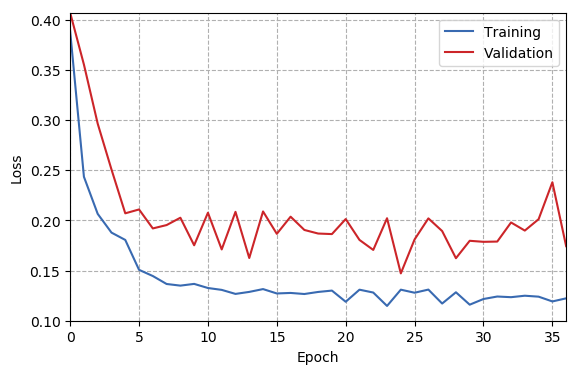
\includegraphics[width=\textwidth]{img/resnet18_all_loss}
        \caption{ResNet18, cross-entropy loss.\label{fig:resnet_loss}}
        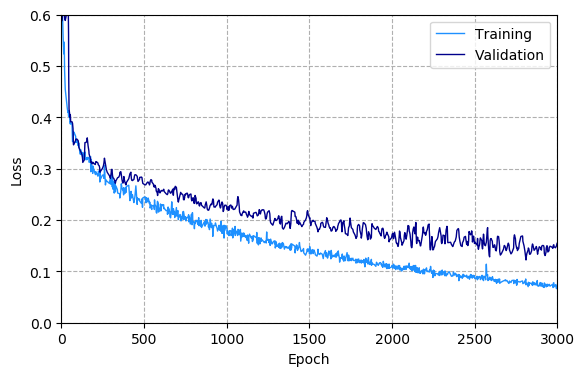
\includegraphics[width=\textwidth]{img/segnet_all_loss}
        \caption{SegNet, cross-entropy loss.\label{fig:segnet_loss}}
    \end{subfigure}
    \begin{subfigure}[t!]{0.5\textwidth}
    	\centering
        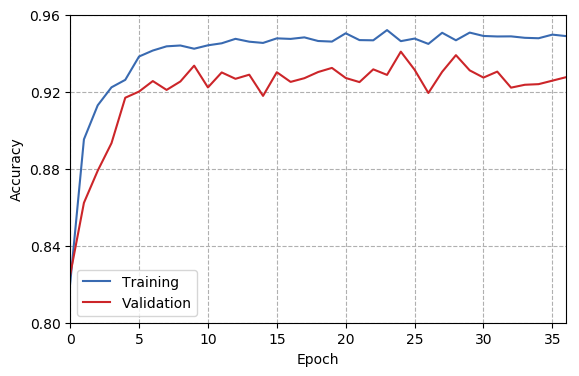
\includegraphics[width=\textwidth]{img/resnet18_all_acc}
        \caption{ResNet18, accuracy.\label{fig:resnet_accuracy}}
        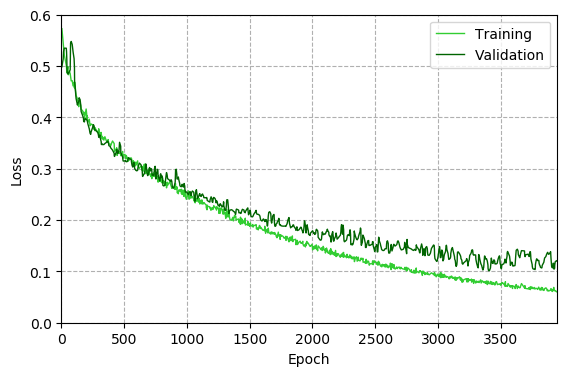
\includegraphics[width=\textwidth]{img/rednet50_all_loss}
        \caption{RedNet50, cross-entropy loss.\label{fig:rednet50_loss}}
    \end{subfigure}
    \caption{Training metrics}
    \label{fig:training_metrics}
    \end{minipage}
    \enspace
	\begin{minipage}[t!]{.195\textwidth}
    \begin{subfigure}[t!]{\textwidth}
        \centering
        \vspace*{.3\baselineskip}
        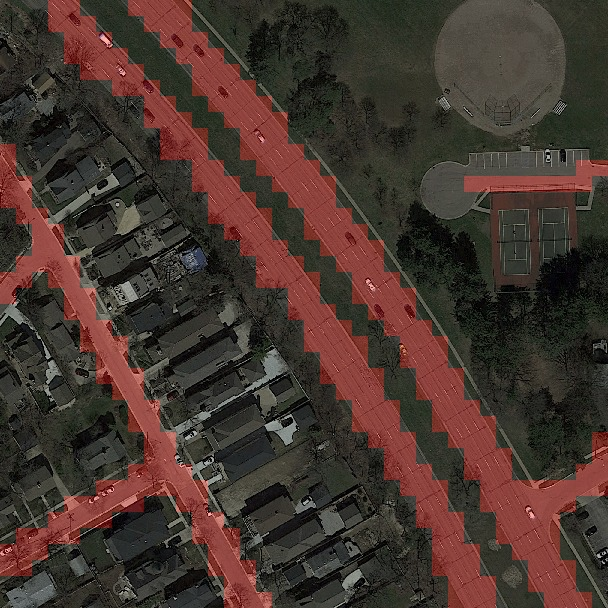
\includegraphics[width=\textwidth]{img/perfect}
        \vspace*{-.5\baselineskip}
        \caption{\!High accuracy.\label{fig:highacc_prediction}}
        \vspace*{1.2\baselineskip}
        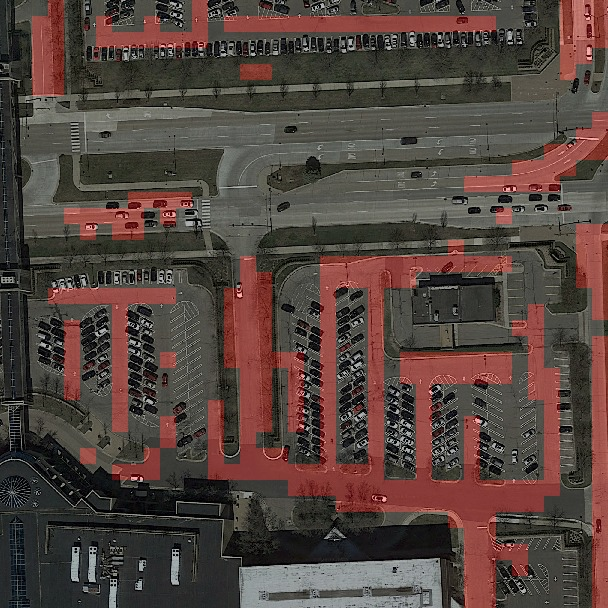
\includegraphics[width=\textwidth]{img/ok}
        \vspace*{-.5\baselineskip}
        \caption{Low accuracy.\label{fig:lowacc_prediction}}
    \end{subfigure}
    \caption{ResNet18 predictions}
    \label{fig:predictions}
    \end{minipage}
    \vspace*{-\baselineskip}
\end{figure*}

Table \ref{tab:kaggle} summarises public and private F\textsubscript{1}-scores for our networks in comparison to baseline networks. The private scores were not available until after the end of competition. The public score is 49\% of the test data and the private 51\%.

\subsection{Metrics}
\label{subsec:metrics}
Figures \ref{fig:resnet_loss}, \ref{fig:segnet_loss} and \ref{fig:rednet50_loss} visualize observed cross-entropy losses for ResNet18, SegNet and RedNet50 respectively. \Cref{fig:resnet_accuracy} shows the accuracy for ResNet18.

\subsection{Segmentation Examples}
\label{subsec:segmentation-examples}
We show a high accuracy prediction of our proposed network in \Cref{fig:highacc_prediction} and use \Cref{fig:lowacc_prediction} for further discussion.


\section{Discussion}
\label{sec:discussion}
\subsection{Kaggle Scores}
Overall, the received scores are similar for segmentation and classification networks. We can conclude that they exhibit similar performance and all three give better results compared to simpler CNNs and are superior to linear classifiers. The better scores are expected, although their similarity leaves room for further research in what hyper-parameters lead to better scores. A significant difference between ResNet18 and segmentation networks is the training time. ResNet18 trained in 5.2h on a GTX670 whereas SegNet took 16.3h and RedNet50 21.7h on a GTX1080Ti.

\subsection{Cross-Entropy Loss}
Comparing the cross-entropy losses from our networks at the respective epochs when they were evaluated shows low correlation to Kaggle F\textsubscript{1}-scores. Comparing losses between two network types is not advised due to different scoring approaches.

When comparing SegNet and RedNet50 where the loss is calculated similarly, these scores are hard to explain and show the use of cross-entropy loss alone to be an unsatisfactory indicator. Using a weighting for the classes ``road'' and ``non-road'' may have been beneficial as the F\textsubscript{1}-score on Kaggle seems to employ such an approach as can be seen in \Cref{tab:kaggle} where marking all patches ``road'' gives a much lower F\textsubscript{1}-score than marking all patches ``non-road''. This behavior was unexpected and was discovered after the end of the competition.

In all networks, it can be seen that the respective models have not exhibited overfitting as the validation loss is still decreasing. Introducing new image data to train on would have likely resulted in fitter models compared to using augmented images. Furthermore, the difference in training and test image dimensions is noteworthy as less data is available to learn on than to predict. This poses an additional challenge and requires solid data augmentation techniques to result in generally fit networks.

\subsection{Double Optimizer}
There are insignificant gains in Figures \ref{fig:resnet_loss} and \ref{fig:resnet_accuracy} on the validation and training set. Implementing the algorithm as explained in \cite{DBLP:journals/corr/abs-1712-07628} could have resulted in better scores yet it proved difficult to implement with Keras. More investigation on relevant hyper-parameters is recommended for ResNet18.

\subsection{Predictions}
\Cref{fig:lowacc_prediction} is particularly interesting as predictions on the large asphalt highway are marking most of it as background yet parts of the concrete parking area are seen as roads. In the former case, it was already mentioned that low amounts of asphalt roads were observed in the training set and as such most roads being misclassified as background by our network. This can be counteracted by modifying the training set to include more of these roads such that the network can learn from them. In the latter case, this brings up another observation that parking spaces sometimes are classified to include roads in the training set, but in other cases not. Therefore, it is unsurprising that our networks struggle with the task. The labeling of parking areas is inconsistent.

\subsection{Network Types}
\subsubsection{Classification Networks}
The main idea of this approach is to utilize CNNs from image classification that perform well. In order to use them, it is necessary to tile the original images both in the training and test sets into patches of fixed size (in our case $16 \times 16$) and perform binary classification on the patch. The benefit is that images of varying sizes can be fed to the network given that the dimensions are multiples of the patch size. A disadvantage of patch-wise classification is the loss of granularity compared to pixel-granular predictions. The resulting predictions allow less post-processing and sometimes appear too coarse.

\subsubsection{Segmentation Networks}
Alternatively, a fully convolutional network that employs an encoder-decoder approach can be used. The encoder-part downsamples the input with convolutions or max-pooling and the decoder upsamples the image back to its original dimensions.

The main advantage of this approach is the pixel-wise granularity of the predictions, concretely each pixel has two logistic units each representing the probability of being ``road'' or ``not road''. Fully convolutional approaches have been shown useful in tasks where very detailed objects exist. In the context of road segmentation, thin roads are predictable with this approach. However, this benefit is questionable as predictions are needed to be performed on patches. Moreover, more non-linearities can be trained with this approach as the complete image is used instead of patches with context.

An unfortunate disadvantage is that it is impractical to input parts of images as this results in different scalings of roads. Additionally, processing patches independently and stitching the results together may lead to unclean stitching artifacts. Furthermore, these networks are of very high dimensionality and therefore training them is a more complex task and finding sensible hyper-parameters is non-trivial and time consuming.

\section{Summary}
\label{sec:summary}
We have shown that with the given road segmentation data classification-based and segmentation-based CNNs perform similarly. Thus, for similar problems, we propose the use of a modified ResNet18 trained with two optimizers as it performed similarly compared to much more complex networks that require more time and involvement to find good hyper-parameters. We expect that overall the performance of all proposed networks can be improved with more varying training images and by finding more appropriate hyper-parameters. We expect the use of post-processing on network-predictions to result in higher accuracies. An interesting approach would be to do this post-processing using another neural network as road design and placement is highly variable.

\clearpage

\bibliographystyle{IEEEtran}
\bibliography{bibliography}

%\includepdf{./declaration_of_independence.pdf}

\end{document}
